
%%%%%%%%%%%%%%%%%%%%%%%%%%%%%%%%%%%%%%%%%%%%%%%%%%%%%%%%%%%%%%%%%%%%%%%%%%%%
%%%%%%%%%%%%%%%%%%%%%%%%%%%%%%%%%%%%%%%%%%%%%%%%%%%%%%%%%%%%%%%%%%%%%%%%%%%%
%%%%                                                                    %%%%
%%%%    Ce fichier contient toutes les parties du document              %%%%
%%%%    Il en détermine aussi l'ordre d'apparition sur le PDF           %%%%
%%%%    Le contenu se trouve dans les dossiers 1, 2 et 3 du projet      %%%%
%%%%    Divisées en 3 parties (Frontmatter, Mainmatter et Endmatter)    %%%%
%%%%    Frontmatter: Parties liminaires paginées en chiffres romains    %%%%
%%%%    Mainmatter: Les parties constituant le corps du texte           %%%%
%%%%    Endmatter: Parties finales (Annexes, médiagraphie, etc.)        %%%%
%%%%                                                                    %%%%
%%%%%%%%%%%%%%%%%%%%%%%%%%%%%%%%%%%%%%%%%%%%%%%%%%%%%%%%%%%%%%%%%%%%%%%%%%%%
%%%%%%%%%%%%%%%%%%%%%%%%%%%%%%%%%%%%%%%%%%%%%%%%%%%%%%%%%%%%%%%%%%%%%%%%%%%%

\pagenumbering{gobble}
    
%%% DÉBUT DES PAGES LIMINAIRES (FRONTMATTER) %%%
    
    % Changement des noms des sections
    \renewcommand\contentsname{TABLE DES MATIÈRES}
    \renewcommand\listfigurename{LISTE DES FIGURES}
    \renewcommand\listtablename{LISTE DES TABLEAUX}
    \newcommand\listofacronymsname{LISTE DES ACRONYMES}
    
    % Page titre
    
%%%%%%%%%%%%%%%%%%%%%%%%%%%%%%%%%%%%%%%%%%%%%%%%%%%%%%%%%%%%%%%
%%%%      Ce fichier contient les fonctions présentes      %%%%
%%%%    Sur la page titre. Il n'y a rien à modifier ici    %%%%
%%%%%%%%%%%%%%%%%%%%%%%%%%%%%%%%%%%%%%%%%%%%%%%%%%%%%%%%%%%%%%%

%%% TITLE PAGE %%%
\thispagestyle{empty}

\begin{center}
    \deptname\\
    \facname\\
    \univname
\end{center}

\vspace*{\fill}

\begin{center}
	\textit{\projecttitle}
\end{center}

\vspace*{\fill}

\begin{center}
    Par \authname
\end{center}

\vspace*{\fill}

\begin{center}
    \profname\\
    \classname
\end{center}

\vspace*{\fill}

\begin{center}
    \cityname\\
    \duedate
\end{center}

\newpage

    % Débuter la numérotation en chiffres romains
    \pagenumbering{roman}
    \setcounter{page}{1}

    % Résumé
    \chapter*{Résumé/Remerciements}
\thispagestyle{empty}

Voici comment insérer une page de résumé et/ou de remerciements avant la table des matières, sans qu'elle apparaisse dans la table des matières, et sans qu'elle ait de numéro de page.

\newpage
    
    % Remerciements
    \chapter*{Résumé/Remerciements}
\thispagestyle{empty}

Voici comment insérer une page de résumé et/ou de remerciements avant la table des matières, sans qu'elle apparaisse dans la table des matières, et sans qu'elle ait de numéro de page.

\newpage
    
    % Table des matières
    \begin{spacing}{1.75}
        \tableofcontents
    \end{spacing}
    
    % Liste des figures
    \cleardoublepage
    \phantomsection
    \addcontentsline{toc}{chapter}{\listfigurename}
    \listoffigures
    
    % Liste des tableaux
    \cleardoublepage
    \phantomsection
    \addcontentsline{toc}{chapter}{\listtablename}
    \listoftables
    
    % Liste des acronymes
    \cleardoublepage
    \phantomsection
    \addcontentsline{toc}{chapter}{\listofacronymsname}
    %%% LISTE DES ACRONYMES %%%
\chapter*{LISTE DES ACRONYMES}

% Write the acronyms here
\begin{acronym}\itemsep=-5pt
    \acro{CA}{Canada}
    \acro{US}{États-Unis}
    \acro{MX}{Mexique}
\end{acronym}

\newpage
    
    \clearpage
    
%%% FIN DES PAGES LIMINAIRES %%%




\pagenumbering{arabic}





%%% DÉBUT DU CORPUS DU TEXTE (MAINMATTER) %%%
    
    % Insérer les chapitres et/ou les sections constituant le corps du texte en ordre ici
    % Voici une représentation des niveaux de section possibles
% Premier niveau
\section{Introduction}\label{section1}

Voici un exemple de section. On peut référencer à une section ou un objet qui a été défini par la fonction \verb|\label{nom du label ici}| en utilisant ensuite la fonction \verb|\ref{label ici}| comme suit (\ref{section1}). 

Voici un exemple de citation d'article de périodique en note de bas de page.\autocite[36]{Periodique2021}

Voici aussi un exemple de citation d'un rapport en note de bas de page.\autocite[579]{Rapport2021}


    \newpage
% Section (premier niveau)
\section{Exemple de section (premier niveau)}

Voici une deuxième section qui sert à démontrer comment faire une note de bas de page explicative en utilisant la fonction \verb|\footnote{texte en note de bas de page ici}| comme suit.\footnote{Insérer le texte qui doit être en note de bas de page ici.}

% Sous-section (second niveau)
\subsection{Exemple de sous-section (second niveau)}

Voici un exemple de sous-section (donc de second niveau). À noter que les numéros des sections et sous-sections se suivent et découlent.

Voici aussi un exemple de citation d'un article de quotidien en note de bas de page.\autocite{Quotidien2021}
    
% Sous-sous-section (troisième niveau)
\subsubsection{Exemple de sous-sous-section (troisième niveau)}

Voici un exemple de sous-sous-section qui suit le même principe que la sous-section précédente.

Voici un exemple de citation de thèse de doctorat ou de mémoire de maitrise en note de base de page. \autocite[50]{These2021}

Voici un exemple de citation d'ouvrage de référence en note de base de page.\autocite{References2021}

% Comment incorporer des acronymes/abréviations
Le \ac{CA}, les \ac{US} et le \ac{MX} sont trois pays d'Amérique du Nord. Ce fut effectué avec la fonction \verb|\ac{CA}, \ac{US}, \ac{MX}|.
    \newpage
\section{Exemples de tableau et figure}



% Comment incorporer une image au texte
\begin{figure}[H]
    \centering
    \caption{Exemple d'image provenant du dossier "images"}
    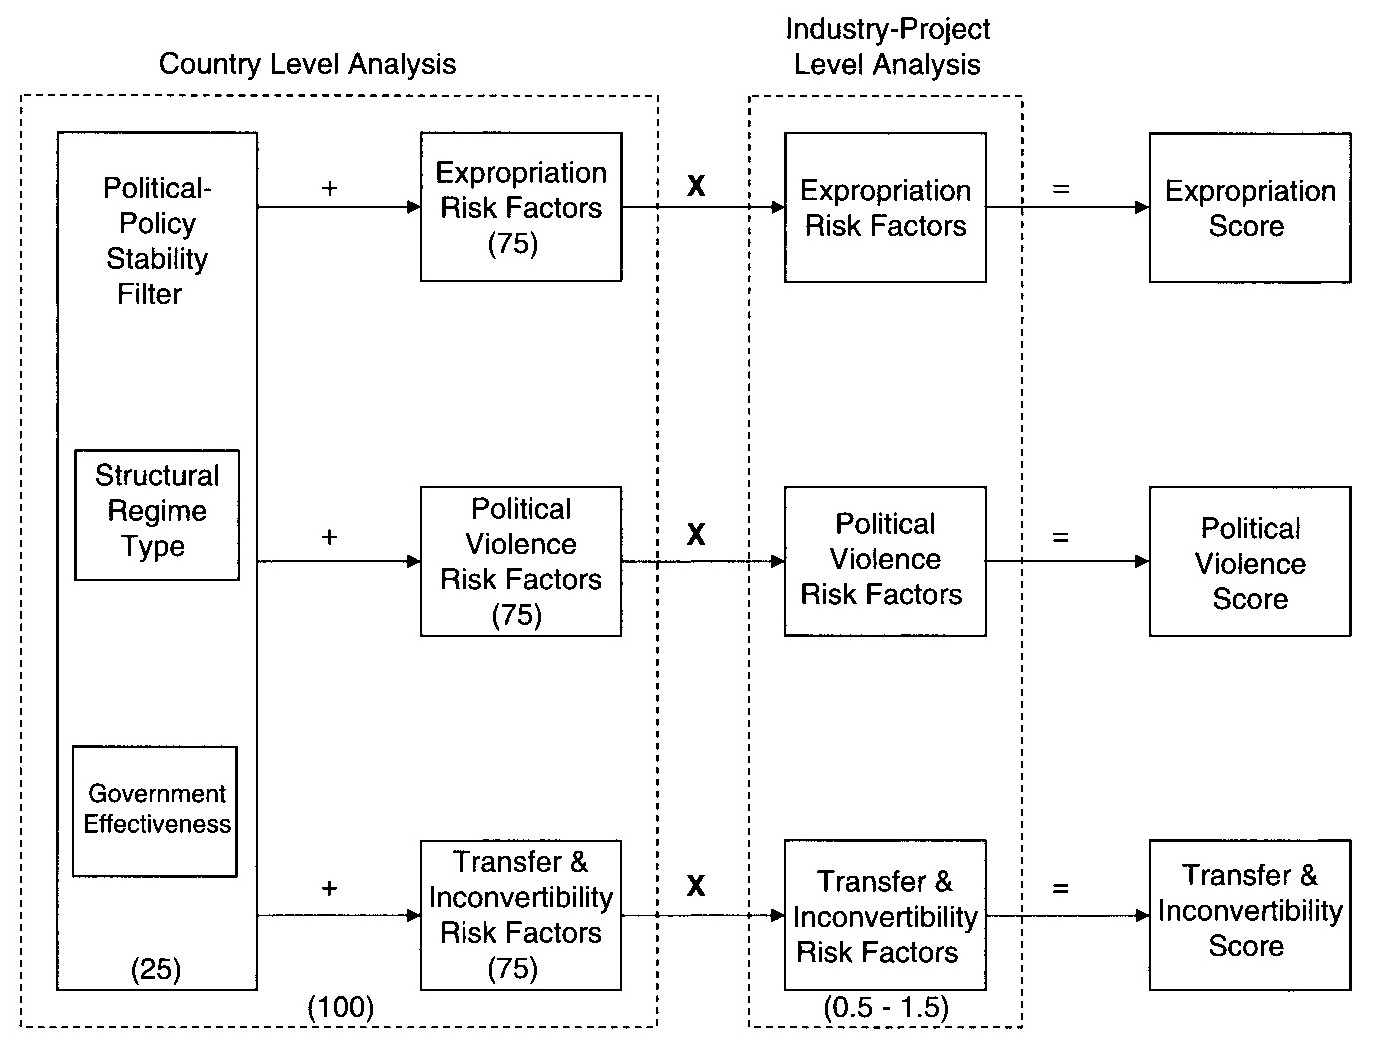
\includegraphics[keepaspectratio, width = 0.75\textwidth]{images/Schema-General.jpg}
    \source{Écrire le nom de la source en texte} % Affiche la note de référence
    \label{figure1} % Une étiquette qui permettra de référer au tableau avec un lien
\end{figure}




% Exemple de tableau
\begin{table}[ht]
    \centering % Centre le tableau dans la page
    \caption{Nonlinear Model Results}\label{tableau1} % Titre et label
    \begin{tabular}{c c c c} % Permet de créer 4 colonnes centrées
        \hline\hline \\ [-6.5ex] % Insère une ligne horizontale double
        Case & Method-1 & Method-2 & Method-3 \\ [0.5ex] % Titres des colonnes
        \hline \\ [-4.5ex] % Insère une ligne horizontale simple
        1 & 50 & 837 & 970 \\ % Insère le corps du tableau
        2 & 47 & 877 & 230 \\ % chaque colonne est séparée par un &
        3 & 31 & 25 & 415 \\
        4 & 35 & 144 & 2356 \\
        5 & 45 & 300 & 556 \\ [1ex] % Ajoute un espace vertical de "1ex" avant la ligne du bas
        \hline % Insère une ligne horizontale simple
    \end{tabular}
    
    \source{Insérer la source des données ici} % Affiche la note de référence
\end{table}
    \section{Conclusion}

Voici une quatrième section qui fait office de conclusion. Si le travail comporte plus ou moins de sections, seulement créer de nouveau fichiers ".tex" ou en effacer dans le sous-dossier "sections" du dossier "2-mainmatter".

Voici une référence à une loi ou règlement en note de bas de page.\autocite{Pays/Etat2021}

    
%%% FIN DU CORPUS DU TEXTE (MAINMATTER) %%%





%%% DÉBUT DES PAGES DE FIN (ENDMATTER) %%%
    
    % Début des annexes
    \begin{appendices}
    \titleformat{\chapter}[display]{\center\fontsize{14pt}{14pt}\selectfont}{\appendixname\ \thechapter}{0pt}{\MakeUppercase}
    
    % Insérer les fichiers d'annexe en ordre ici
    \chapter{EXEMPLES DE LISTES ET BOÎTES DE TEXTE}

% Exemple de liste en points
Exemple de liste en points
\begin{itemize}
  \item La liste commence par la fonction \verb|\begin{itemize}| et chaque objet (point) de la liste commence par la fonction \verb|\item|.
  \item Chaque objet de la liste commence par un point automatiquement placé.
  \item Le texte de chaque objet peut être de n'importe quelle taille.
  \item La liste doit OBLIGATOIREMENT se terminer par la fonction \verb|\end{itemize}|
\end{itemize}

% Exemple de liste ordonnée

Exemple de liste ordonnée
\begin{enumerate}
  \item La liste commence par la fonction \verb|\begin{enumerate}| et chaque objet (chiffre) de la liste commence par la fonction \verb|\item|.
  \item Les objets de la liste sont ordonnés et le chiffre est apposé automatiquement.
  \item Le texte de chaque objet peut être de n'importe quelle taille.
  \item La liste doit OBLIGATOIREMENT se terminer par la fonction \verb|\end{enumerate}|
\end{enumerate}

% Exemple de boîte de texte

Deux exemples de boîtes de texte :

Une boîte de texte avec fond gris/parchemin

\begin{textbox_parchemin}{Titre de la boîte de texte}
    Entrer le texte qui doit être dans la boîte ici. Cette longue ligne de texte permettra de vérifier l'interligne qui change à l'intérieur de la boîte, par rapport au corps du texte.
\end{textbox_parchemin}

Une boîte de texte avec fond blanc

\begin{textbox_blanc}{Titre de la boîte de texte}
    Entrer le texte qui doit être dans la boîte ici.
    \\
    \\
    La boîte supporte des sauts de ligne.
    \\
    \\
    \\
    \\
    Mais aussi.
    \\
    \\
    \\
    \\
    Les sauts de page.
    \\
    \\
    \\
    \\
    Sans briser la boîte.
\end{textbox_blanc}
    % \input{3-endmatter/Annexe-B}
    % \input{3-endmatter/Annexe-C}
    % \input{3-endmatter/Annexe-D}
    % \input{3-endmatter/Annexe-E}
    
    % Fin des annexes
    \end{appendices}

    % Médiagraphie (après OU avant les annexes)
    \singlespacing
    \printbibliography[heading=bibintoc, title=\vspace{6pt}MÉDIAGRAPHIE]
    
%%% FIN DES PAGES DE FIN (ENDMATTER) %%%